\hypertarget{sec:justification}{%
\chapter{Model Justification}\label{sec:justification}}

The verification results of a model have no bearing on TreeKEM unless the model is a faithful and equivalent translation of the protocol.
To verify the TreeKEM protocol, the CGKA security game is used.
Proof that the TreeKEM protocol is a CGKA protocol, as well as proof that results of the CGKA security game for any CGKA protocol are valid for FS and PCS, have already been produced \autocite{alwen2020security}.
Justifying the equivalence of this work's modeling of both the CGKA security game and the side channel attacker knowledge gained while observing the TreeKEM protocol, is pivotal to the soundness of verifying FS and PCS for TreeKEM.

Within this chapter we will formalize a parameterized model \CGKAmod{P}{T}{N}.
For a given LTL predicate $\varphi$ we define \CGKAmod{P}{T}{N} as follows:

\[
\begin{split}
\CGKAmod{P}{T}{N}\quad\models\quad& \varphi \textrm{ iff }\quad\forall t \in [1, T],\, n \in [2, N], c \in [1, T]\\
  & \varphi \textrm{ holds in all possible \CGKAsec\!s}\\
  & \textrm{with a \CGKAdef complatible protocol } \mathtt{P}\\
  & \textrm{played by an } (t, c, n)\textrm{-attacker}
\end{split}
\]

\hypertarget{sec:game-adaptations}{%
\section{CGKA game formalization}\label{sec:game-adaptations}}

Many novel techniques were used when formalizing the abstractly defined CGKA security game to a rigorous and model suitable for explicit state model checking.
The CGKA security game is originally defined informally as a massively concurrent game, without a bounded win condition as shown in Figure \ref{fig:CGKA-informal}.
This is not always problematic for explicit state model checking, but regrettably it is with regards to CGKA security game.

Within the CGKA game the attacker makes a series of queries to the available oracles.
Queries to oracles drive the CGKA protocol's state over time, however, when playing the game as originally defined there are no guaranteed limits on total attacker queries to all oracles.
Furthermore, while the attacker decides exactly which order to query which oracles, all group members of the CGKA protocol concurrently broadcast an unlimited number of messages, both informational and control.
A direct modeling of the CGKA game with a \((T, C, N)\)-attacker would require \(N+1\) concurrent processes, accounting for the attacker and the maximum possible group members, along with \(N\) infinite queues of messages to be received by participants, and crucially monotonically increasing epoch and message counters representing the total ordering enforced by the delivery service.
A single state in the state-space would constitute the unique combination of all actor processes' internal states, all message queue states, and the global protocol state.
Unfortunately, because of the monotonically increasing counters, there can be no finite representation of the infinite game.

To construct a finite model of an unbounded game, the states of the model must not have depend on any monotonically increasing temporal information.
Temporal information which converges to a limit in finitely many steps or converges to a to a finite cycle in finitely many steps can all be finitely modeled.
If a model's state depends on non-converging temporal information, it necessitates that the state-vector length and search-space are unbounded.
This follows from the following three facts.

\begin{enumerate}
\def\labelenumi{\arabic{enumi}.}
\item
  Each state in the state-space must have a unique state-vector encoding.
\item
  The model's state and the equivalent state-vector's encoding must include monotonically increasing temporal information.
\item
  In an unbounded game, there is no finite encoding of monotonically increasing temporal information.
\end{enumerate}

While explicit state model checking is sophisticated, it ultimate reduces to an exhaustive search which uses a myriad of techniques to cleverly reduce the search space.
There does not exist an general technique for reducing an unbounded, potentially infinite, search space to a finite one, as this would yield a solution to the halting problem.
Considerable thought was given towards identifying a specific unbounded-to-finite reduction for the CGKA security game, but the author is unable to present such a technique in this work.
Instead, different techniques are presented to ``truncate'' an equivalent finite ``prefix'' of the CGKA security game.
In terms of a \((T, C, N)\)-attacker \(\mathcal{A}\), verification is performed from epochs $0$ to \(T_{max}\), truncating the CGKA security game to all prefix sequences containing at most \(T_{max}\) epochs.

The model of CGKA security game for the TreeKEM protocol described subsequently in this chapter, is be parameterized by $t \in \{ 0, T_{max} \}$.
Model parameterization by $t$ means that the CGKA security game is played until epoch $t$ is reached, at which point play continues \emph{without} advancing to epoch $t+$, with the attacker eventually ending the game with a call to \Oracle{deliver}{}.
Verification for the finite \CGKAsec prefixes less than or equal to \(T_{max}\) requires $|\{ 0, T_{max} \}|$ seperate verification runs, one for verifying the CGKA model parameterized by each possible $t$ value with $t \in \{ 0, T_{max} \}$.
While simple and effective, this approach does involve duplicate verification work, with the verification of the model for $t$ being an optimal substructure for verifying the model parameterized by $t+1$.
The work presented here does not attempt memoization of sub-problems, though this is theoretically and practically possible with additional engineering effort.

\begin{figure}
  \centering
  \caption{\label{fig:CGKA-informal}Transition graph of informal CGKA definition}
  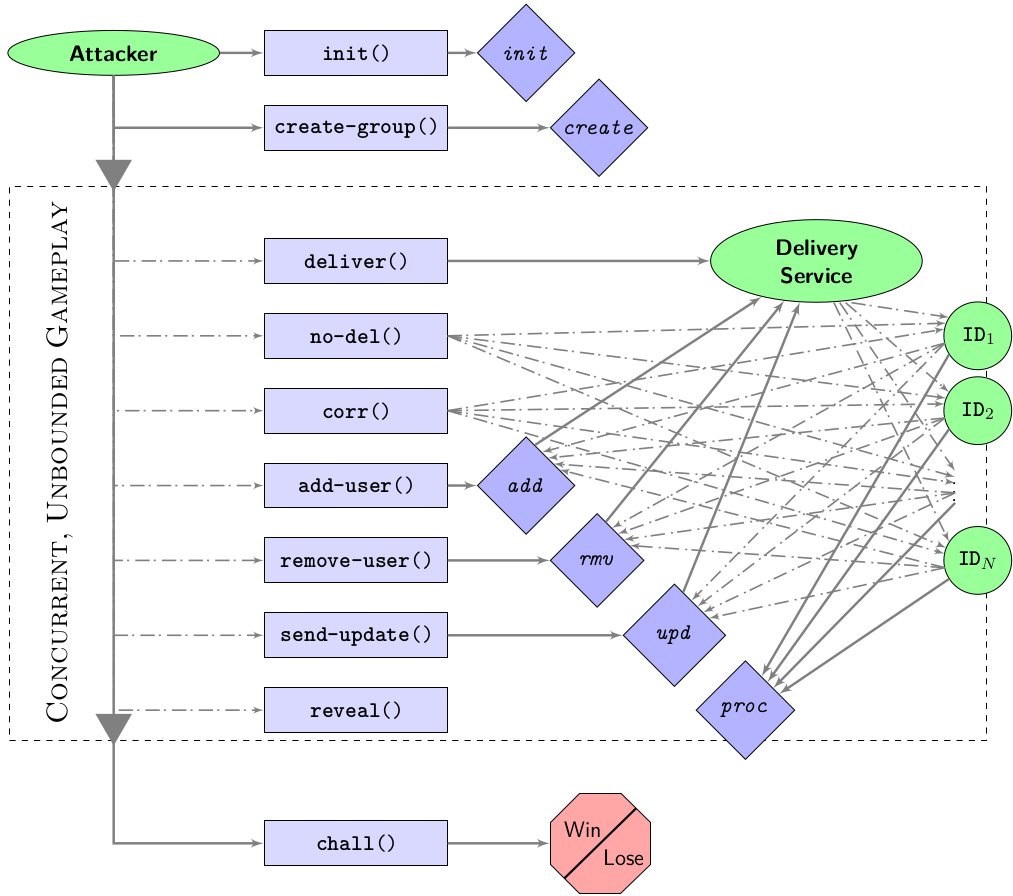
\includegraphics[width=\textwidth]{figures/CGKA-informal.png}
\end{figure}

\hypertarget{exhaustiveness}{%
\subsection{Exhaustiveness}\label{exhaustiveness}}

Verification through explicit state model checking relies on exhaustiveness as it's proof method.
However, the definition of the CGKA security game had no notion of considering every possible interleaving of actions when created.
Instead, it was defined in a manner which made existential proofs easy to describe and reason about.
Proofs and counterexamples from previous works \autocite{alwen2019double}, \autocite{alwen2020security} take the form of scrutinizing the existence of a sequence of queries made by the attacker.
This existential focus permits leniency for redundancy within the CGKA security game definition.
Conversely, modeling the CGKA security game such that it is amenable to explicit state model checking demands absolute parsimony within definition.
Considering the CGKA games definition through the lens an exhaustive state-space search, both conveniently and surprisingly, leads to many possible game simplifications.
Because all states are considered, equivalent or superfluous sequences can be reasoned about, identified, and collapsed.

Consider the parameter \(C\) for a \((T, C, N)\)-attacker \(\mathcal{A}\).
As defined, in each epoch \(\mathcal{A}\) must perform exactly one of the following:

\begin{itemize}
  \item Query \Oracle{reveal}{} exaclty once.
  \item Query \Oracle{chall}{}  exaclty once.
  \item Query niether \Oracle{reveal}{} or \Oracle{chall}{}.
\end{itemize}

Additionally, to terminate the \CGKAsec, \(\mathcal{A}\) must query \Oracle{chall}{} once.
Therefore, for all \((T, C, N)\)-attacker \(\mathcal{A}\), \(C \in [1, T]\).
Because the exhaustive state space of is explored, at each epoch the attacker chooses one of the three explicit querying options related to \Oracle{reveal}{} and \Oracle{chall}{}.
Hence within the model \CGKAmod{P}{T}{N}, the parameter \(C\) is linearly dependant on \(T\) for all \((T, C, N)\)-attackers and does not need to be a model parameter.
Similar reductions will follow while formalizing \CGKAmod{P}{T}{N} from the informal \CGKAsec definition.

\hypertarget{idempotence}{%
\subsection{Idempotence}\label{idempotence}}

A literal interpretation of the informal \CGKAsec definition permits many redundant state transitions.
Importantly idempotent operations are permitted.
For a sequence of operations \( \{ o_0 \circ o_{1} \circ \ldots \circ o_{m-1} \circ o_{m} \} \), and idempotent operation \(q\) is one in which \(q = q \circ q = q \circ p \circ q\) for all subsequences \(p = \{o_i \ldots o_j \} \in \{ o_0 \circ o_{1} \circ \ldots \circ o_{m-1} \circ o_{m} \} \).
Similarly, for all sequences of operations containing an idempotent operation \(q\), between every operand in the sequence after the first occurance of \(q\), an additional occurance of \(q\) can be inserted without effecting the result of the operations.
As shorthand, we will denote \(q \circ p \gets q^{*}\) to represent the expansion of a sequence \(p\) containing an idempotent operation \(q\) into the set of all sequences \(p\) with possible insertions of additional \(q\) opertations into \(p\).
It will be clear to an attentive reader that the cardinality of \(q \circ p \gets q^{*}\) is countably infinite, as it follows the same logical construction of the rational numbers.

The concept of idempotency phrased in the context of a stateful protocol modeled as a transittion graph, relates an idempotent operation \(q\) as one in which, performing \(q\), then at a later point while in state \(s\) performing \(q\) again, results in a cycle from \(s\) to \(s\).
This is probelematic for an exhaustive search.
Quite obviously it permits an infinite loop in within \CGKAmod, which in turn makes certain LTL statement impossible to verify as well as increasing the verification runtime.
The following are examples of permitted idempotency by the informal \CGKAsec definition:

\begin{itemize}
  \item For some \(t\), the attacker querries \Oracle{reveal}{t}    two or more times throught the \CGKAsec.  
  \item For some \(i\), the attacker querries \Oracle{no-del}{ID_i} two or more times throught the \CGKAsec.
  \item For some \(i\), and some \(t\), the attacker querries \Oracle{corr}{ID_i} two or more times during epoch \(t\).
\end{itemize}

Since the verification methodology for \CGKAmod{P}{T}{N} exhuastively explores all possible \CGKAsec states, all sequences of operations \(q \circ p \gets q^{*}\) are equivelent.
Hence we can collapse the cyclical search through the countably infinite number of idempotent sequences, considering them all to be the same unique state without effecting the verification of an LTL property \(\varphi\).
To disallow the cycles formed by idempotent operations, each operation above is permitted only once per period within which the operation is idempotent.
Within the \CGKAmod Promela encoding, repeated sequences of idempotent operations are tabulated within the global game state and guarded against.
By disallowing idempotency within the game, each query made by the attacker will never result in a return to a previous game state.
A consequence of this, is that attacker queries necissarily advance the game state towards the next epoch tranision, or when within the final epoch, advance towards the query to \Oracle{chall}{}.
This necissarily progression of the \CGKAsec within the model \CGKAmod{P}{T}{N} both reduces the runtime verification as well as permits verification that the model \CGKAmod{P}{T}{N} halts.

\hypertarget{elided-group-members}{%
\subsection{Elided Group Members}\label{elided-group-members}}

The complexity of the asynchronous, multi-party communication described by the informal \CGKAsec definition is illistrated within Figure \ref{fig:CGKA-informal}.
However, exhaustiveness can once again reduce model complexity.
Consider a \((T, C, N)\)-attacker \(\mathcal{A}\).
As defined, in each epoch $t < T$ the transition from epoch $t$ to epoch $t+1$ can only occur in one of the following ways:

\begin{itemize}
  \item For some \(i\), \(\mathtt{ID_i}\) calls \Protocol{add} and subsequently \(\mathcal{A}\) queries \Oracle{deliver}{t,\, ID_i,\, ID_{*} }
  \item For some \(i\), \(\mathtt{ID_i}\) calls \Protocol{rmv} and subsequently \(\mathcal{A}\) queries \Oracle{deliver}{t,\, ID_i,\, ID_{*} }
  \item For some \(i\), \(\mathtt{ID_i}\) calls \Protocol{upd} and subsequently \(\mathcal{A}\) queries \Oracle{deliver}{t,\, ID_i,\, ID_{*} }
  \item For some \(i\), \(\mathcal{A}\) queries \Oracle{add-user}{ID_i}    then \Oracle{deliver}{t,\, ID_i,\, ID_{*}}
  \item For some \(i\), \(\mathcal{A}\) queries \Oracle{remove-user}{ID_i} then \Oracle{deliver}{t,\, ID_i,\, ID_{*}}
  \item For some \(i\), \(\mathcal{A}\) queries \Oracle{send-update}{ID_i} then \Oracle{deliver}{t,\, ID_i,\, ID_{*}}
\end{itemize}

\hypertarget{decidability}{%
\subsection{Decidability}\label{decidability}}

\hypertarget{sec:game-oracles}{%
\section{Oracles}\label{sec:game-oracles}}

\hypertarget{corrupt}{%
\subsection{Corrupt}\label{corrupt}}

\hypertarget{hoard}{%
\subsection{Hoard}\label{hoard}}

\hypertarget{reveal}{%
\subsection{Reveal}\label{reveal}}

\hypertarget{insert}{%
\subsection{Insert}\label{insert}}

\hypertarget{remove}{%
\subsection{Remove}\label{remove}}

\hypertarget{update}{%
\subsection{Update}\label{update}}

\hypertarget{deliver}{%
\subsection{Deliver}\label{deliver}}

\hypertarget{sec:LTL-security}{%
\section{Security}\label{sec:LTL-security}}

\hypertarget{pcs-as-ltl}{%
\subsection{PCS as LTL}\label{pcs-as-ltl}}

\begin{LTL}[\,PCS\,]
    $$
    \Box \Big(\, ( \texttt{CGKA@start\_of\_epoch} \land \texttt{unsafeIDs} = 0 ) \implies \neg \texttt{learnedKey[epoch]} \Big)
    $$
\end{LTL}

\hypertarget{fsu-as-ltl}{%
\subsection{FSU as LTL}\label{fsu-as-ltl}}

\begin{LTL}[\;Never-Trivial\;]
    $$
    \Box \left( \texttt{CGKA@move\_corrupt} \implies \texttt{hoarding[targetID]} = \texttt{NEVER} \right)
    $$
\end{LTL}

\begin{LTL}[\;FSU-Epoch(\,\textnormal{\normalfont $t \in T$}\,)\;]
    \begin{equation*}
    \begin{split}
    \Diamond ( & \texttt{CGKA@move\_start\_of\_epoch} \land \texttt{epoch} = t + 1 \land \neg \texttt{learnedKey[$t$]} ) \\
    & \implies ( \neg \texttt{learnedKey[$t$]} ) \,\;{\mathcal {U}}\;\, \texttt{CGKA@end\_of\_game}
    \end{split}
    \end{equation*}
\end{LTL}

\begin{LTL}[\;FSU\;]
    $$
    \textbf{Never-Trivial} \implies \bigwedge\limits_{t=0}^{T} \;\,\textbf{FSU-Epoch}(t)
    $$
\end{LTL}
k
